\begin{figure*}[ht!]
\centering
  \begin{subfigure}{0.32\textwidth}
                \centering
    \includegraphics[width=\textwidth]{./fig/co2.eps}
                \caption{$CO_{2}$}
  \end{subfigure}
  \begin{subfigure}{0.32\textwidth}
                \centering
    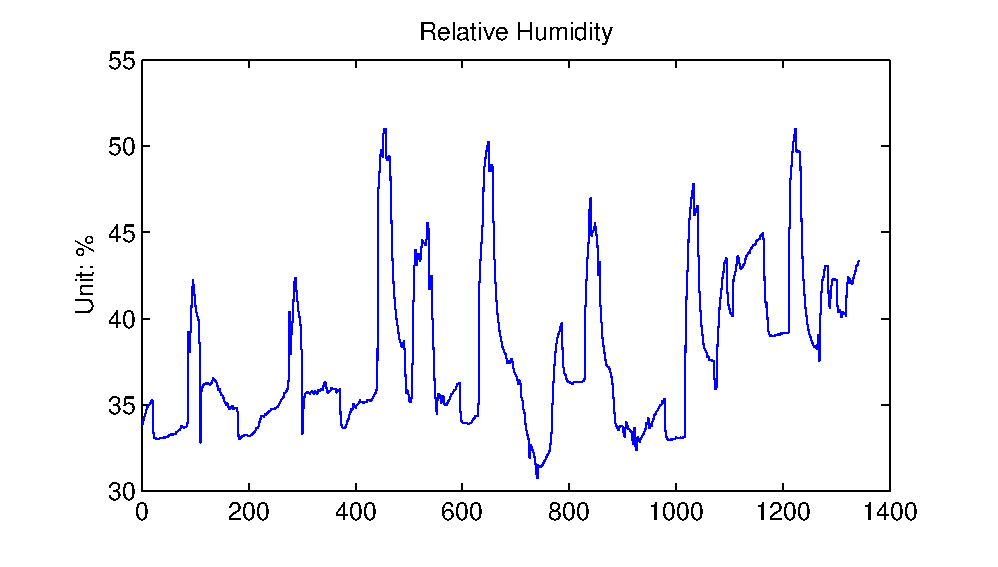
\includegraphics[width=\textwidth]{./fig/rh.eps}
                \caption{Humidity}
  \end{subfigure}
  \begin{subfigure}{0.32\textwidth}
                \centering
    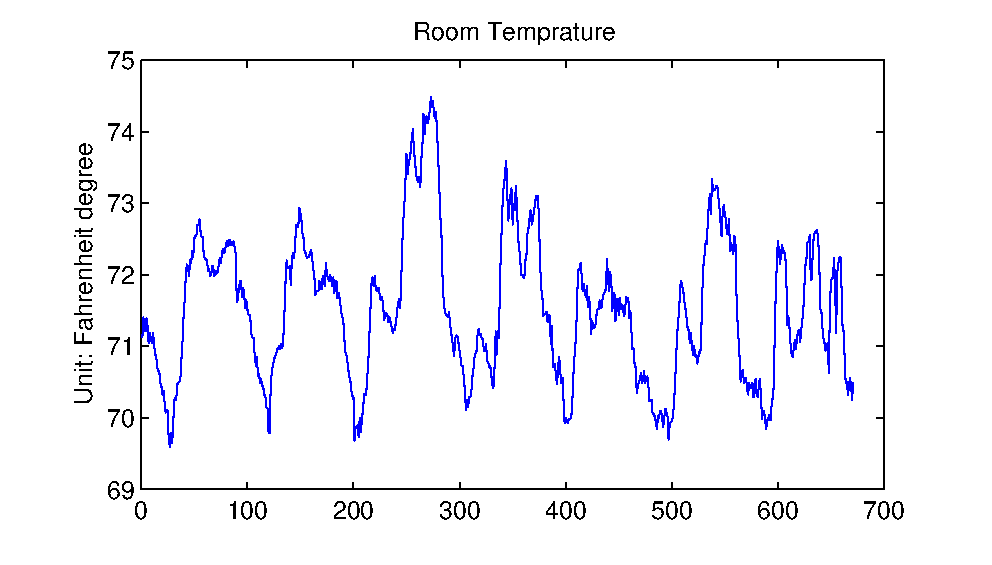
\includegraphics[width=\textwidth]{./fig/rmt.eps}
                \caption{Room Temperature}
  \end{subfigure}
  %row2
  \begin{subfigure}{0.32\textwidth}
                \centering
    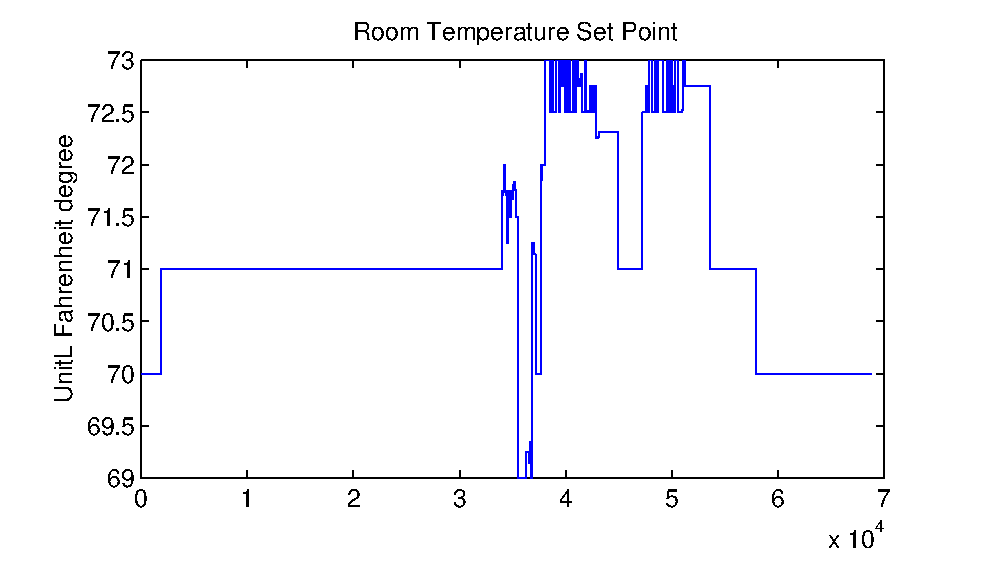
\includegraphics[width=\textwidth]{./fig/stpt.eps}
                \caption{Room Temperature Set Point}
  \end{subfigure}
  \begin{subfigure}{0.32\textwidth}
                \centering
    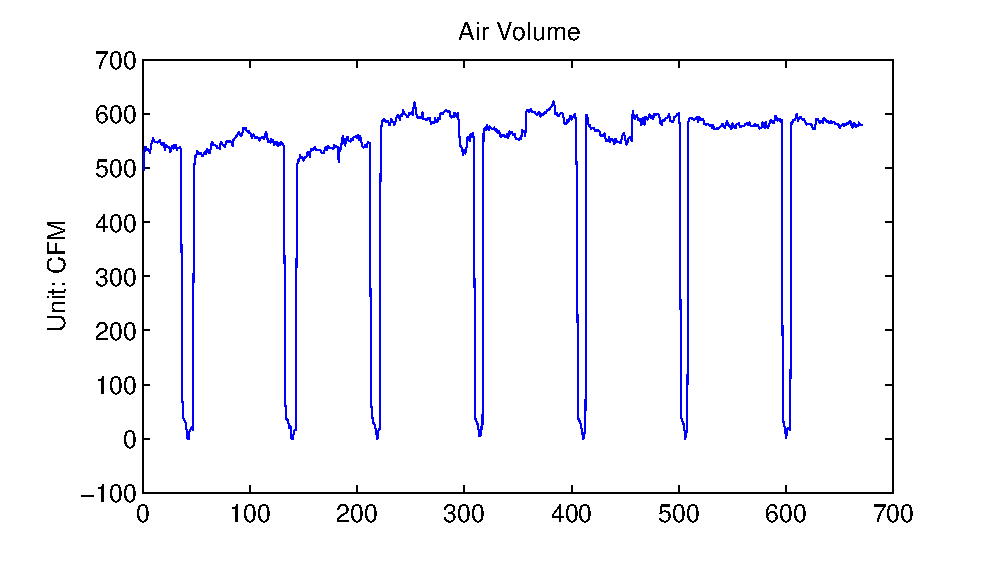
\includegraphics[width=\textwidth]{./fig/vav.eps}
                \caption{VAV Air Volume}
  \end{subfigure}
  \begin{subfigure}{0.32\textwidth}
                \centering
    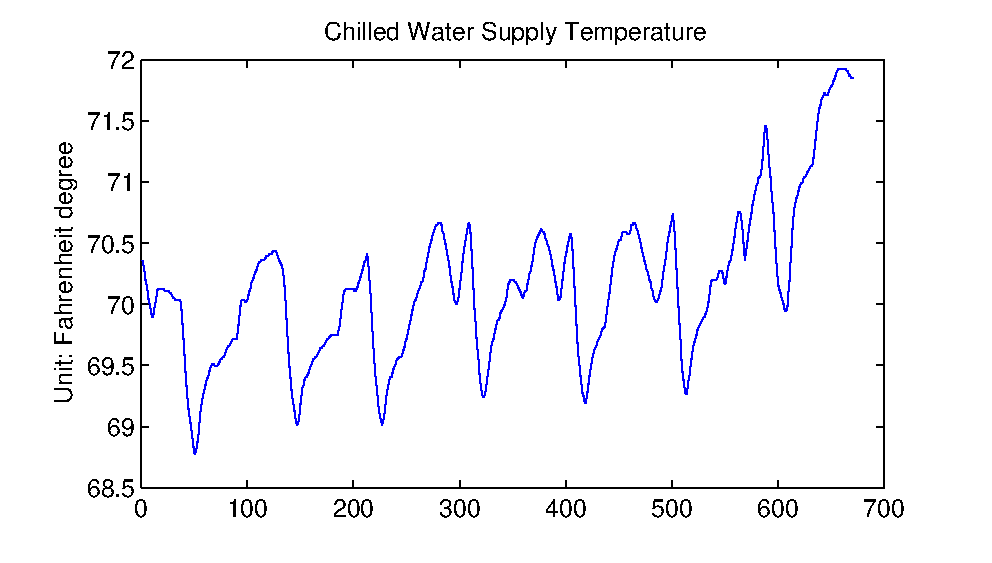
\includegraphics[width=\textwidth]{./fig/cwt.eps}
                \caption{Chilled Water Supply Temperatere}
  \end{subfigure}
\caption{Different type of sensor occupies different amplitude bins in the time domain with different short term dynamics.}
\label{fig:example}
\end{figure*}

\section{Methodology}
In this section, we describe the design and construction of the feature-vector we use to characterize sensor \emph{type}.  We
explain what it captures, fundamentally and, hence, why it works so well for building sensor data. Then, we discuss
the classification technique we apply and give a detailed description of the training and testing process. Finally, we articulate
a solution for identifying potentially misclassified streams, when no type-label ground truth is available.

\subsection{Feature Extraction}
Raw sensor time series\footnote{In this paper, we use the term ``trace'', ``readings'' and ``time series'' \textit{interchangeably}.} usually contain millions of readings which are too general to be useful for type classification.   We need to distill the information embedded in the reading patterns.
A signal in the time domain trends the amplitude of a sensor reading and different types of sensor generally occupy distinct
amplitude bins, as demonstrated in Figure~\ref{fig:example}. We can characterize the amplitude distribution of a signal in the time
domain by using the percentiles of the value distribution.%, such as 25th, 50th, 75th and so forth. 
To identify outliers in the distribution, we pick the 50th percentile value (also known as the median) as a discriminator, which
is more robust to outliers skew than the average. 

% Sensor readings, in particular, are subject to the dynamics in the environment they are deployed in
% therefore sensors of different types can overlap in a same amplitude bin.  
Naturally, sensor reading value-ranges may overlap. For example, during a rainy season, the humidity in an
office can reach the range of 60-70 (percent) which is the same as typical temperature sensor readings (Fahrenheit).
If you do not consider measurement units, the distributions for each of the two types look similar. 
Simply relying on percentiles is not sufficient for differentiating sensor types. Figure~\ref{fig:same_bin} demonstrates this
point. To capture their difference we need to include the variance of the signal in our feature-vector.

\begin{figure}[ht!]
\centering
  \begin{subfigure}{0.22\textwidth}
                \centering
    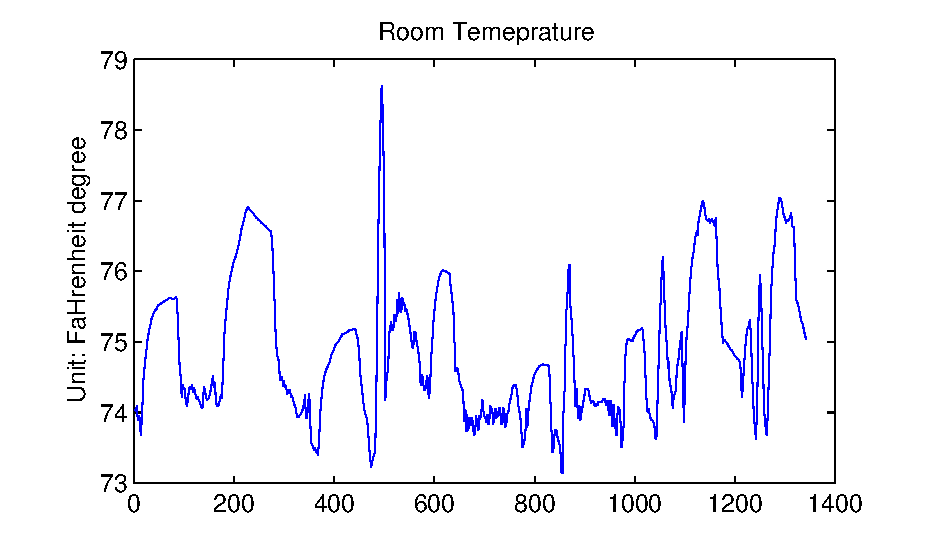
\includegraphics[width=\textwidth]{./fig/rmt_ex.eps}
                \caption{Room Temperature}
  \end{subfigure}
  \begin{subfigure}{0.22\textwidth}
                \centering
    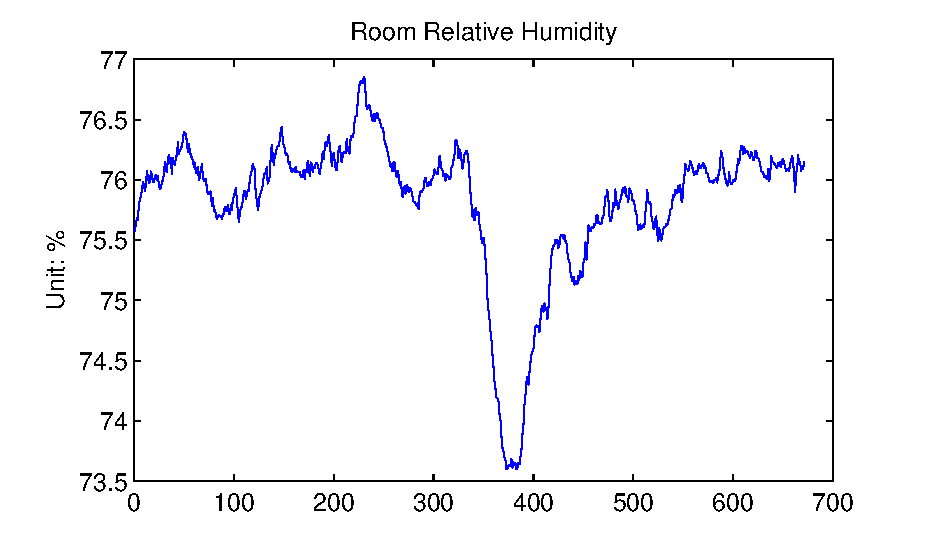
\includegraphics[width=\textwidth]{./fig/rh_ex.eps}
                \caption{Humidity}
  \end{subfigure}
\caption{An example of two differernt type of sensors occupying the same amplitude bin.}
\label{fig:same_bin}
\end{figure}

% When we extract features from a raw sensor reading, the original trace can span over hour, days or even weeks, and the trend can vary significantly even from hour to hour. On
% one side, extracting certain features such as percentiles and variances over the entire sensor reading might miss too many short term dynamics thus making the features less discrimi- nant, compared to doing so in shorter windowed time slices. On the other side, computing features over windowed slices can produce too many elements for a feature vector and also, having too many unnecessary feature variables might degrade the performance of classifier. To better and suc- cintly summarize the dynamics of sensor traces, we apply feature extraction to every time window of fixed length on the original trace and compute the statistics of the accumu- lated features from windowed slices as the final features.

When we extract features from a raw sensor readings, the original trace can span hours, days, or weeks, and
the trend can vary significantly, even from hour to hour. Extracting certain features, such as percentiles, and
variances over the entire sensor trace might miss  short term dynamics thus missing discriminating characteristics.
In contrast, computing features over short time windows can produce too much noise.  Too many  feature variables typically 
degrades classifier performance.
To succinctly summarize the dynamics of sensor traces, we apply feature extraction to every time window of fixed length on 
the original trace and compute the statistics of the accumulated features from windowed slices as the final feature set. 

Upon close inspection of the traces, we notice that the short-term dynamics of the phenomena being measured, could be used
to differentiate them.  Therefore, the distribution of short-term summary statistics can be used discriminate
traces by type.  We construct our feature vector as follows: first,
% As a summary, the feature extraction procedure goes as follows. First, 
each single sensor signal is segmented into N
non-overlapping 45-minute long windows (we will discuss the decision of window length in later section). Second, within
each time window, we compute the median and variance of the signal, producing a vector of medians and a vector of
variances after the window slides over an entire trace: 
\begin{displaymath}
\begin{split}
MED = \{median^{1}, median^{2}, ..., median^{N}\}\\
VAR = \{variance^{1}, variance^{2}, ..., variance^{N}\}
\end{split}
\end{displaymath}
Where N is the number of time windows. The vector $MED$ and $VAR$ reflect short term changes but not all the intermediate values are essentially useful for classification. Finally, we compute a statistical summary of the two vectors.   For each vector we compute the minimum, maximum, median and variance, resulting in a feature vector with eight variables:
\begin{displaymath}
\begin{split}
F = \{min(MED), max(MED), median(MED), var(MED),\\
 min(VAR), max(VAR), median(VAR), var(VAR)\}
\end{split}
\end{displaymath}
And $F$ is the feature vector for each sensor trace used in our classification process.

\subsection{Classification}
% After transforming all sensor time series into feature vectors, we use an ensemble classifier to achieve 
% the type classification. 
In general, ensemble learning methods obtain better predictive performance than
 any of the constituent learning methods as discussed in~\cite{ensem1,ensem2}, if the following assumptions hold~\cite{ensem3}: 1) the 
 probability of a correct classification by each individual classifier is greater than 0.5 and 2) the errors
  in predictions of the base-level classifiers are independent. Random forests~\cite{RF} have been widely used 
  and outperform a single tree classifier. They are also faster~\cite{cvpr} in training and testing compared to traditional classifiers such as SVM. The notion of randomized trees was first introduced in~\cite{RT} and further well developed in~\cite{RF}.

Random forests construct a multiple of classification trees. To classify an unlabeled object, we construct the feature vector and 
``feed'' the vector down each of the trees in the forest. Each tree gives a classification and we use it as a 
``vote" for that class. The forest chooses the class having the most votes over all the trees in the forest. 
% As a quick overview of how each tree is grown in the forest, 
The process proceeds as follows:
\begin{enumerate}
\item Sample N instances at random with replacement\footnote{An element may appear multiple times in the sample set.}, from the original data set. These samples will be the training set for growing this particular tree.
\item Specify M feature variables at random out of the total feature vector when growing each node of a tree. And the best split (measured by the information gain) on these M is used to split the node. The value of M is constant during the forest growing.
\item Each tree is grown to the largest extent possible without pruning.
\end{enumerate}
The randomness of this ensemble learning method occurs in the first two steps.  We set N equal the number of instances in the original training set, M equal the square root of the
number of original feature variables, and the number of the trees in the forest be 50. Usually these parameters are optimized
through cross-validation and we refer interested readers to~\cite{RF} for further deduction and proof of random forest.

All the instances in our data set are labeled with ground truth class. To train a random forest, we split the original set into two subsets, one for building 
a forest and one for testing the accuracy of the classifier. After the forest is built from training set, we learn the posterior probabilities of each class $c$ 
at each leaf node $l$ for each tree $t$: suppose that $T$ is the set of all trees, $C$ is the set of all classes and $L$ is the set of all leaves for a given 
tree $t\in T$. In the training stage the posterior probabilities $P_{t,l}(Y(i) = c))$ for each class $c\in C$ at each leaf $l\in L$, are learned for each tree $t\in T$. 
These probabilities are calculated as \textit{the ratio of the number of instance $i$ of class $c$ that reach $l$ to the total number of intances that reach $l$}. $Y(i)$ 
is the class label for instance $i$. To classify an instance in the testing stage, the feature vector of an instance is passed down each tree until reaching a leaf 
node, which gives a probability distribution. All the posterior probabilities accumulated from each tree are then averaged and the $argmax$ is taken as the class 
of the instance. Note that instead of letting each tree vote for on class as described in the original paper~\cite{RF}, we combine the results from classifiers for 
an instance by averaging their probabilistic predictions, in order to facilitate our technique used to help identify potential misclassified instances as described in the following section.  

% \begin{algorithm}[h!]
%  \SetAlgoLined
%  Give signal $X(t)$:\\
%   \While{the \# of maxima in $X(t)$ >3}{
%   (1) identify all the local extrema in $X(t)$\;
%   (2) perform a cubic spline interpolation of maxima to get the upper envelope\;
%   (3) repeat (2) on minima to get the lower envelope\;
%   (4) $h(t) = X(t) - mean((2),(3))$ \;
%   (5) repeat (2)-(4) until $h(t)$ is an IMF\;
%   (6) $X(t) = X(t) - h(t)$, and return the IMF\;
%   }
%  \caption{Empirical Mode Decomposition}
%  \label{alg:emd}
% \end{algorithm}

\subsection{Quantify Classification Uncertainty}
Being able to measure the confidence of prediction results and to identify potential misclassifications, is vital to a learning process. 
It is trivial to 
identify misclassification when ground truth is available, but in many real-world cases ground truth is unavailable. %labels are not available.
%  Therefore, the 
% efforts to identify potential misclassifications would suffer from the absence of ground truth. 
Quantifying classification uncertainty can help identify potential misclassified instances and presents an opportunity to solicit 
the user for feedback that we can use to improve our results. To quantify the uncertainty of classifications in our learning process, we use
 the posterior probabilities learned in the random forest.

With the learned posterior probabilities for each class, at each leaf in each tree, we can compute the average probabilities 
for each class as follows:
\begin{displaymath}
    \bar P(Y(i)=c) = \frac{\sum_{t} P_{t,l}(Y(i)=c)}{|T^{'}|}, t\in T^{'}
\end{displaymath}
Where $T^{'}$ is the collection of trees in the forest where $P_{t,l}(Y(i)=c)\neq 0$, and $|\cdot|$ denotes the cardinality of a set. Given these averaged 
probabilities for each class, the forest produces a vector of class probabilities for each new instance as:
\begin{displaymath}
\textbf{Pr} = \{\bar P(Y(i)=c)\}, c\in C
\end{displaymath}
Suppose we have a probability vector $Pr_{1} = \{0.9, 0, 0, 0, 0, 0.1\}$ for instance $i_{1}$ and another vector $Pr_{2} = \{0.3, 0.25, 0.1, 0, 0.15, 0.2\}$ for instance $i_{2}$.
Both $i_{1}$ and $i_{2}$ will be assigned to the same class according to the class probability distribution, but the assignment of $i_{2}$ is less confident compared to that 
of $i_{1}$ because its predicted class probability has a less ``concentrated'' distribution. To measure the degree of ``uncertainty'' in classification of one instance, 
we compute the entropy of its class probability yielded by the forest. We rank the classification results and filter out the instances for 
further manual inspection whose entropy are above a threshold.  Inspection can help eliminate misclassifications.
